\documentclass[10pt,letter]{article}

%------------------------------------------------------------------------------------------------------------------------%
\usepackage{blindtext}
%\usepackage[french]{babel} 			% parce qu'on travaille en fraçais
\usepackage[utf8]{inputenc}	% maudit MAC!
%\usepackage[cyr]{aeguill}				% règle un problème de guillemets
\usepackage{amssymb}				% pour les lettres grecques
\usepackage{amsmath}				% plein de bonus pour les maths
\usepackage{amsfonts}				% plein de fonts pour les maths
\usepackage{fullpage} 				% parce qu'on a pas de note en marge
\usepackage{geometry}				% permet de changer les marges
\usepackage[pdftex]{graphicx}		% permet de dimensioner des graphismes
%\usepackage{tocbibind}				% inclut la TOC et la BIBLI dans la table des matière
\usepackage[small,bf]{caption}		% change le format des captions
\usepackage{wrapfig}					% permet de mettre des petite figures en petit
\usepackage{multicol}					% plusieurs colonnes
\usepackage{fancyhdr}				% pour faire des beaux headers
\usepackage[pdftex,plainpages=false,colorlinks=true,linkcolor=blue, citecolor=blue, urlcolor=blue]{hyperref}
\usepackage{fancyvrb}
\usepackage{natbib}
%\usepackage{titlesec}
\usepackage{blkarray}


\setlength{\parskip}{\baselineskip}%
\setlength{\parindent}{0pt}%

% pretty tilde:
%\usepackage{times}
%\usepackage{textcomp}
%

\usepackage{listings}
\usepackage{xcolor}
\usepackage{color}
\usepackage[framemethod=tikz]{mdframed}
\usepackage{verbatim}

\definecolor{myletters}{rgb}{1.0,0.972,827}
\definecolor{mymauve}{rgb}{0.262,0.098,0.188}
\definecolor{mycomment}{rgb}{0.315,0.47,0.74}
\definecolor{myblue}{rgb}{0.098,0.188,0.262}
\definecolor{myred}{rgb}{1.0,0.3,0.1}

%\definecolor{myletters}{rgb}{0.0,0.0.3,0.0}
%\definecolor{mymauve}{rgb}{0.97,0.95,0.97}
%\definecolor{mycomment}{rgb}{0.315,0.47,0.74}
%\definecolor{myblue}{rgb}{1.0,1.0,1.0}
%\definecolor{myred}{rgb}{1.0,0.3,0.1}


\newcommand{\dollar}{\mbox{\textdollar}}
\newcommand{\vdollar}{\texttt{\$}}



\newmdenv[hidealllines=true,
  backgroundcolor=mymauve,
  leftmargin=10pt,
  rightmargin=20pt,  
  innerleftmargin=-5pt,
  innerrightmargin=-5pt,
  innertopmargin=2pt,
  innerbottommargin=2pt,
  roundcorner=5pt,
  nobreak=true]{bashInput}


\newmdenv[hidealllines=true,
  backgroundcolor=myblue,
  leftmargin=10pt,
  rightmargin=10pt,  
  innerleftmargin=-5pt,
  innerrightmargin=-5pt,
  innertopmargin=2pt,
  innerbottommargin=2pt,
  roundcorner=5pt,
  nobreak=true]{bashInput2}


\newmdenv[hidealllines=true,
  backgroundcolor=mymauve,
  leftmargin=10pt,
  rightmargin=10pt,  
  innerleftmargin=-5pt,
  innerrightmargin=-5pt,
  innertopmargin=10pt,
  innerbottommargin=2pt,
  roundcorner=5pt,
  nobreak=true]{bashInput3}


\lstset{columns=fullflexible,basicstyle=\ttfamily}


\lstdefinestyle{BashInputStyle}{
  language=bash,
  basicstyle=\small\ttfamily\color{myletters},
  frame=none, 
  backgroundcolor=\color{mymauve},
  linewidth=0.9\linewidth,
  xleftmargin=0.1\linewidth,
  commentstyle=\color{mycomment},
  columns=flexible,
  showstringspaces=false,
  moredelim=**[is][\color{myred}]{~@}{@~},
  mathescape = true
}

\lstdefinestyle{BashInputStyle2}{
  language=bash,
  basicstyle=\small\ttfamily\color{myletters},
  frame=none, 
  backgroundcolor=\color{myblue},
  linewidth=0.9\linewidth,
  xleftmargin=0.1\linewidth,
  commentstyle=\color{mycomment},
  columns=flexible,
  showstringspaces=false,
  moredelim=**[is][\color{myred}]{~@}{@~},
  mathescape = true
}


\lstset{columns=fullflexible,basicstyle=\ttfamily}


%----------------------------------------------------------------------%

\setlength{\oddsidemargin}{25mm}
\setlength{\evensidemargin}{25mm}
\setlength{\voffset}{-1in}
\setlength{\hoffset}{-1in}
\setlength{\textwidth}{166mm}
\setlength{\topmargin}{4mm}
\setlength{\headheight}{10mm}
\setlength{\headsep}{12mm}
\setlength{\topskip}{0mm}
\setlength{\textheight}{228mm}

\pagestyle{fancy}
\makeatletter
\newenvironment{tablehere}
  {\def\@captype{table}}
  {}
\newenvironment{figurehere}
  {\def\@captype{figure}}
  {}
\makeatother



\fancyhead[LO,LE]{Maxime Charlebois}
\fancyhead[RO,RE]{Inchworm: implementation notes}


\begin{document}
\title{Diagram analysis}
\author{M. Charlebois$^{1}$}
\date{\today}

%\maketitle

\newcommand{\bra}[1]{\langle #1 \vert}
\newcommand{\ket}[1]{\vert #1 \rangle}
\newcommand{\braket}[2]{\langle #1 \vert #2 \rangle}



Notes on the implementation of the inchworm in triqs.

\section{Diagram notation}


From Gull review:
\begin{align}
U(\beta)=& \operatorname{Tr_B} [e^{-\beta (H_a + H_\text{hyb}) }]  
\\
=&  \sum_{k=0}^{\infty} \int_{0}^{\beta} d \tau_{1} \cdots \int_{\tau_{k-1}}^{\beta} d \tau_{k} \int_{0}^{\beta} d \tau_{1}^{\prime} \cdots \int_{\tau_{k^{\prime}-1}}^{\beta} d \tau_{k}^{\prime} \\
& \times \operatorname{Tr_B}\left[T_{\tau} e^{-\beta H_{a}} \tilde{H}_{\mathrm{hyb}}\left(\tau_{k}\right) \tilde{H}_{\mathrm{hyb}}^{\dagger}\left(\tau_{k}^{\prime}\right) \cdots\right. \left.\times \tilde{H}_{\mathrm{hyb}}\left(\tau_{1}\right) \tilde{H}_{\mathrm{hyb}}^{\dagger}\left(\tau_{1}^{\prime}\right)\right]
\end{align}

where
$H_{\mathrm{hyb}}=\sum_{p j}\left(\theta_{p}^{j} c_{p}^{\dagger} d_{j}+\theta_{p}^{j *} d_{j}^{\dagger} c_{p}\right)=\tilde{H}_{\mathrm{hyb}}+\tilde{H}_{\mathrm{hyb}}^{\dagger}$. Then: 
\begin{align}
U(\beta)=& \sum_{k=0}^{\infty}   \int_{0}^{\beta} d \tau_{1} \cdots \int_{\tau_{k-1}}^{\beta} d \tau_{k} \int_{0}^{\beta} d \tau_{1}^{\prime} \cdots \int_{\tau_{k-1}^{\prime}}^{\beta} d \tau_{k}^{\prime} \\
& \times \sum_{j_1^{(\prime)} \cdots j_k^{(\prime)}} \sum_{p_1^{(\prime)} \cdots  p_k^{(\prime)}} 
\theta_{p_{1}}^{j_{1}} \theta_{p_{1}^{\prime}}^{j_{1}^{\prime}*} \cdots \theta_{p_{k}}^{j_{k}} \theta_{p_{k}^{\prime}}^{j_k^{\prime}*} \\
& \times \operatorname{Tr_B}\left[T_{\tau} e^{-\beta H_{a}} d_{j_{k}}\left(\tau_{k}\right) c_{p_{k}}^{\dagger}\left(\tau_{k}\right) c_{p_{k^{\prime}}}\left(\tau_{k}^{\prime}\right)   d_{j_{k}^{\prime}}^{\dagger}\left(\tau_{k}^{\prime}\right) \right.\\
&\left. \cdots d_{j_{1}}\left(\tau_{1}\right) c_{p_{1}}^{\dagger}\left(\tau_{1}\right) c_{p_{1}^{\prime}}\left(\tau_{1}^{\prime}\right) d_{j_{1}^{\prime}}^{\dagger}\left(\tau_{1}^{\prime}\right)\right]
\end{align}

With and $H_a=H_\mathrm{loc}+H_\mathrm{bath}$ we can reorder: 
\begin{align}
U(\beta)=& \sum_{k=0}^{\infty}  \int_{0}^{\beta} d \tau_{1} \cdots \int_{\tau_{k-1}}^{\beta} d \tau_{k} \int_{0}^{\beta} d \tau_{1}^{\prime} \cdots \int_{\tau_{k-1}^{\prime}}^{\beta} d \tau_{k}^{\prime} \\
& \times \sum_{j_1^{(\prime)} \cdots j_k^{(\prime)}} \sum_{p_1^{(\prime)} \cdots  p_k^{(\prime)}} 
\theta_{p_{1}}^{j_{1}} \theta_{p_{1}^{\prime}}^{j_{1}^{\prime}*} \cdots \theta_{p_{k}}^{j_{k}} \theta_{p_{k}^{\prime}}^{j_k^{\prime}*} \\
& \times \left[T_{\tau} e^{-\beta H_{\mathrm{loc}}} d_{j_{k}}\left(\tau_{k}\right) d_{j_{k}^{\prime}}^{\dagger}\left(\tau_{k}^{\prime}\right) \cdots d_{j_{1}}\left(\tau_{1}\right) d_{j_{1}^{\prime}}^{\dagger}\left(\tau_{1}^{\prime}\right)\right] \\
& \times \operatorname{Tr_B}\left[ e^{-\beta H_{\mathrm{bath}}} c_{p_{k}}^{\dagger}\left(\tau_{k}\right) c_{p_{k^{\prime}}}\left(\tau_{k}^{\prime}\right) \cdots c_{p_{1}}^{\dagger}\left(\tau_{1}\right) c_{p_{1}^{\prime}}\left(\tau_{1}^{\prime}\right)\right]
\end{align}


We define the hybridization partition of the bath (with $k$ electron) as:
\begin{align}
Z_{\mathrm{bath}}=\operatorname{Tr} e^{-\beta H_{\mathrm{bath}}}=\prod_{\sigma} \prod_{p}^k \left(1+e^{-\beta \epsilon_{p}}\right)
\end{align}

For every electron $p$, the energy is given by:
\begin{align}
\Delta_{l m}(\tau)=\sum_{p} \frac{\theta_{p}^{l *} \theta_{p}^{m}}{e^{\epsilon_{p} \beta}+1} \times\left\{\begin{array}{ll}
{-e^{-\epsilon_{p}(\tau-\beta)},} & {0<\tau<\beta} \\
{e^{-\epsilon_{p} \tau},} & {-\beta<\tau<0}
\end{array}\right.
\end{align}

Then (I need to think about it more):
\begin{align}
\frac{1}{Z_{\text {bath }}} \operatorname{Tr_B}\Big[T_{\tau} e^{-\beta H_{\text {bath }}} \sum_{p_1 \ldots p_k}  \sum_{p_{1}^{\prime} \ldots p_k^{\prime}} 
\theta_{p_{1}}^{j_{1}} \theta_{p_{1}^{\prime}}^{j_{1}^{\prime} *} \cdots \theta_{p_{k}}^{j_{k}} \theta_{p_{k}^{\prime}}^{j_{k}^{\prime}*}  
\\
\quad \times c_{p_{k}}^{\dagger}\left(\tau_{k}\right) c_{p_{k^{\prime}}}\left(\tau_{k}^{\prime}\right) \cdots c_{p_{1}}^{\dagger}\left(\tau_{1}\right) c_{p_{1}^{\prime}}\left(\tau_{1}^{\prime}\right)\Big]=\operatorname{det} \Delta
\end{align}
Ok, I need to do this proof at least once. 

Using this last definition, we get:
\begin{align}
U(\beta)=& Z_{\text {bath }} \sum_k^{\infty} \int_{0}^{\beta} d \tau_1 \cdots \int_{\tau_k}^{\beta} d \tau_k^{\prime}
\\
&\sum_{j_1 \ldots j_k}  \sum_{j_{1}^{\prime} \ldots j_k^{\prime}} 
\Big[ T_{\tau} e^{-\beta H_\mathrm{loc}}
d_{j_k}(\tau_k) d_{j_k^\prime}^{\dagger} (\tau_k^\prime) \cdots d_{j_1}(\tau_1) d_{j_1^\prime}^{\dagger} (\tau_1^\prime) \Big] \operatorname{det} \Delta
\end{align}




Zeroth order: 
\begin{align}
U_0(\beta)=& Z_{\text {bath }} e^{-\beta H_\mathrm{loc}}
\end{align}

First order: 
\begin{align}
U_1(\beta)=& Z_{\text {bath }} \int_{0}^{\beta} d \tau_1 \int_0^{\beta} d \tau_1^{\prime}
\sum_{j_1 j_1^\prime}  
\Big[ T_{\tau} e^{-\beta H_\mathrm{loc}}
d_{j_1}(\tau_1) d_{j_1^\prime}^{\dagger} (\tau_1^\prime) \Big] \Delta_{j_1 j_1^\prime} ( \tau_1 - \tau_1^\prime)
\end{align}

For an extremely simple case (one site, $U=0$, $H_\text{loc}=0$, one bath $\epsilon=0$, $\Delta=-\frac{\theta^2}{2}$):
\begin{align}
U_1(\beta) / U_0(\beta)=& -\frac{(\beta \theta)^2}{2}
\end{align}

\pagebreak


This simple system can be solved exactly
\begin{align}
U(\beta)=& \operatorname{Tr_B} [e^{-\beta (H_\text{loc} + H_\text{bath} + H_\text{hyb}) }]  
\end{align}

\pagebreak

\begin{align} 
U(\beta)=& \operatorname{Tr_B} [e^{-\beta (H_a + H_\text{hyb}) }]  
\\
U(\beta)=&  \text{Tr}_B\left[
\sum_{k} \frac{1}{k !} 
\sum_{a b} 
e^{-\beta H_\text{loc}}
\int_{0}^{\beta} 
\prod_{i=1}^{k} d \tau_{i} d \tau_{i}^{\prime} 
c_{b_i}\left(\tau_{i}^{\prime}\right)    
\Delta_{a_i b_i}\left(\tau_{i} - \tau_{i}^{\prime}\right)   
c_{a_i}^{\dagger}\left(\tau_{i}\right) 
\right]
\end{align}

propagator:


A diagram is a compact way to represent the equations:
\begin{align} 
To 
\\
be
\\ 
done
\end{align}

In the following two sections, we will explore the formalism used here along a simple example that can be generated with the code \url{https://github.com/TRIQS/inchworm.git} under the tag \Verb#doc_0.1# (commit number \Verb#d0745e5#). After building with \Verb#cmake#, run in the file \Verb#build_directory/test/c++/diagram_analysis# to generate the example below.

\section{Proper diagrams}

\label{sec::proper}

%Suppose a time $\tau_{split}$, 

An hybridization line is considered crossing with $\tau_{c}$ if $\Delta_{ab}(\tau,\tau^\prime)$ has $\tau < \tau_{c} < \tau^\prime$ or  $\tau > \tau_{c} > \tau^\prime$. An hybridization line is considered connected if it is crossing with either a split time $\tau_{split}$ or one and only one between of the two times ($\tau$ and $\tau^\prime$) of at least one other connected hybridization line. And a diagram is considered proper if every of its hybridization are connected to a split time.

To find this, we need to implement a simple deep first search algorithm. We start by listing all $\Delta_{ab}(\tau-\tau^\prime)$  that cross $\tau_{split}$, and from these, successivly search all the $\Delta_{ab}(\tau,\tau^\prime)$ that are connected. This deep first search algorithm is simple, but let's consider an example. Let's consider that after ordering in time the creation an annihilaiton operator, we obtain the chain $c(\tau_0)c^\dagger(\tau_1)c(\tau_2)c^\dagger(\tau_3)c^\dagger(\tau_4)c(\tau_5)c^\dagger(\tau_6)c(\tau_7)$ where time are ordered ($\tau_i<\tau_{i+1}$).  Only the order of operator matter here, so this information can be summarized with the diagram like \Verb#x-o-x-o-o-x-o-x#. 

Now suppose a split time $\tau_{split}$ such that $\tau_5 < \tau_{split} < \tau_6$. We need to find, for a distribution of hybridization line if a diagram is proper or not. Note that there is one hybridization per $c(\tau)$ and $c^\dagger(\tau^\prime)$, i.e. as much as the order of expansion $n$. Also, there $n!$ way to connect the different $c(\tau)$ and $c^\dagger(\tau^\prime)$ with hybridization lines, hence $n!$ different diagrams to analyse. For the example here $n=4$ hence there is  $24$ different configurations to consider. Let's take and analyse one of these diagrams. On these graph here, an hybridization line (either \Verb#...#, \Verb#___# or \Verb#===#) is represented under the diagram \Verb#x-o-x-o-o-x-o-x#, and it shows which \Verb#o# and \Verb#x# are linked.


\noindent\begin{minipage}[t]{.5\textwidth}
\begin{bashInput3}
\begin{lstlisting}[style=BashInputStyle]
diagram no.19:  permutation (3 0 1 2 )
            |    
x-o-x-o-o-x-o-x
  _____________ 
.......         
    .....       
           ___   
          
notation: ___ is crossing split time
           ... not crossing split time
\end{lstlisting}   
\end{bashInput3}
\end{minipage}\hfill
\begin{minipage}[t]{.5\textwidth}
\begin{bashInput3}
\begin{lstlisting}[style=BashInputStyle]
after deep first search:
            |    
x-o-x-o-o-x-o-x
  ============= 
=======         
    =====       
           ===   
          
notation: === is connected to split time
           ... not connected to split time
\end{lstlisting}   
\end{bashInput3}
\end{minipage}

This example diagram chosed here is considered proper since every hybridization line are connected to the split time. Indeed, if you start from the first hybridization line, which is crossing the split point (vertical line), we see that the second one is crossing with the first time of the first hybridization line. After the third one is crossing with the second time of the second hybridization line. The last one is crossing with the split time already. Hence in the end, the diagram is proper. Let's consider another configuration of hybridizations:

\noindent\begin{minipage}[t]{.5\textwidth}
\begin{bashInput3}
\begin{lstlisting}[style=BashInputStyle]
diagram no.20:  permutation (3 0 2 1 )
            |    
x-o-x-o-o-x-o-x
  _____________ 
.......         
         ...     
     _________   

notation: ___ is crossing split time
           ... not crossing split time
\end{lstlisting}   
\end{bashInput3}
\end{minipage}\hfill
\begin{minipage}[t]{.5\textwidth}
\begin{bashInput3}
\begin{lstlisting}[style=BashInputStyle]
after deep first search:
            |    
x-o-x-o-o-x-o-x
  ============= 
=======         
         ...     
     =========   

notation: === is connected to split time
           ... not connected to split time
\end{lstlisting}   
\end{bashInput3}
\end{minipage}
Again, following the same procedure from above, we see that it is evident that the third hybridization line is not connected, hence this configuration is not proper.

Note that this definition of connectivity is different from the one defined usually in the inchworm reference papers. This is a little technical for now, but we intend to use the dressed propagator on both side of the split points, hence not every point on the right side of the split point are connected by default. This is the only difference. But it will also affect the inclusion-exclusion method presented in the next section.


\section{Inclusion-exclusion}
\label{sec::inclu}

This is a very brief summary of the algorithm. It is composed of two important classes: \Verb#segment# and \Verb#set_of_segment# and three important lists: a vector of single \Verb#segment#, a vector of \Verb#set_of_adjacent_segments# and a vector of \Verb#set_of_disjoint_segments#.


\noindent\begin{minipage}[t]{.5\textwidth}
\begin{bashInput3}
\begin{lstlisting}[style=BashInputStyle]
list of single segements:
            |    
x-o-x-o-o-x-o-x
=== -----------
======= -------
=========== ---
- === ---------
--- === -------
--- ======= ---
------- === ---
----------- ===
===============
\end{lstlisting}   
\end{bashInput3}

\begin{bashInput3}
\begin{lstlisting}[style=BashInputStyle]
list of set of adjacent segments:
            |    
x-o-x-o-o-x-o-x
=== === -------
=== ======= ---
======= === ---
--- === === ---
=== === === ---

\end{lstlisting}   
\end{bashInput3}

\end{minipage}\hfill
\begin{minipage}[t]{.5\textwidth}

\begin{bashInput3}
\begin{lstlisting}[style=BashInputStyle]
list of set of disjoint segments:
            |    
x-o-x-o-o-x-o-x
=== -----------
======= -------
=========== ---
- === ---------
--- === -------
--- ======= ---
------- === ---
----------- ===
===============
=== --- === ---
=== ------- ===
======= --- ===
=========== ===
- === - === ---
- === ----- ===
--- === --- ===
--- ======= ===
------- === ===
=== --- === ===
- === - === ===
\end{lstlisting}   
\end{bashInput3}
\end{minipage}


The vector of \Verb#segment# lists all the single segments possible on this diagram. A  \Verb#segment# must contain the same number of \Verb#o# (creation operator) and \Verb#x# (annihilation operator), and it must not cross a split point (vertical line on the graph). \Verb#===# lines represent segments and \Verb#---# lines represent the rest of the diagram that is not as segment.

From this list we can generate the two other lists by combining every possible segment, successively. If they are all adjacent, it is pushed back in the vector \Verb#set_of_adjacent_segments# and if they are all disjoint, it is pushed back in the vector of \Verb#set_of_disjoint_segments#. These three vectors are necessary and sufficient to calculate the value associated with every single \Verb#segment#.

We start by calculating the value of the smaller segments as any \Verb#segment# depends only on the value of \Verb#segment# smaller than itself, and the smallest segments are trivial to calculate. 

The value of a single \Verb#segment# ($S$) can be calculated in two steps, first calculate the value without adjacent segment (or value without cuts in the source code), noted $c_k(V)$ (or \Verb#+++# sign in the graphs below) and the value with adjacent segments (or value in source code), noted $a_k(S)$ (or \Verb#===# sign in the graphs below) from these two equations:
\begin{align} 
\label{c_S}
c(S) &=\sum_{j} (-1)^{P(R^j)}  v(R^j) \prod_{i}\left[-a(D^j_{i})\right]
\\
\label{a_S}
a(S) &=\sum_{j} \prod_{i}\left[-c(A^j_{i})\right]
\end{align}
where $D^j_{i}$ represent the $i^{th}$ individual segment in the $j^{th}$ \Verb#set_of_disjoint_segments#, $A^j_{i}$  represent the $i^{th}$ individual segment in the $j^{th}$ \Verb#set_of_adjacent_segments#, and finally $R^j = S \backslash \bigcup_{i} D^j_{i}$ is the remainder of the of the vertices in the segment $S$ that are not included in any segment $D^j_{i}$ for the $j^{th}$ \Verb#set_of_disjoint_segments#. $v(R^j)$ is the determinant of the hybridization difference matrix of the remainding indices $R^j$.

Note that the sign $ (-1)^{P(R^j)}$ is important and missing from the paper of~\cite{boag_inclusion-exclusion_2018}. This sign is non trivial. The number $P(R^j)$ corresponds to the number of permutations that would be required to reunite all the indices in $R^j$ into a continuous segment at the rightmost position of the segment $S$.

Let's take an example of a specific segment: the third segment of the first list (shown above), since it is long and non trivial. This segment define the range $[0,6[$. 

For the calculation of $c(S)$ (Eq~\eqref{c_S}) we need to refer to the list of set of disjoint segments above: every \Verb#set_of_disjoint_segments# that enter into the range $[0,5[$ must be considered. Note that we need to exclude the \Verb#set_of_disjoint_segments# that overlap with the last vertex since we need to calculate the fully connected segment (see Boad et al. 2018 for details, for now at least). We use the value $a(S)$ from the previously calculated smaller segments, calculate the sign $ (-1)^{P(R^j)}$ and the determinant $v(R^j)$ of the remainding indices, and thus calculate Eq~\eqref{c_S}.

For the calculation of $a(S)$ (Eq~\eqref{a_S}) we need to refer to the list of set of adjacent segments above: every \Verb#set_of_adjacent_segments# that have exactly the same range $[0,6[$ must be considered. We use the value $c(S)$ from the previously calculated smaller segments and thus calculate Eq~\eqref{a_S}. We show the segment used from the list above for the segment example considered here:

\noindent\begin{minipage}[t]{.5\textwidth}
\begin{bashInput3}
\begin{lstlisting}[style=BashInputStyle]
Calculation of value of c(S):
               |    
   x-o-x-o-o-x-o-x
   +++++++++++
=
   -----------
-  === -------
-  ======= ---
+  - === -----
-  --- === ---
\end{lstlisting}   
\end{bashInput3}
\end{minipage}\hfill
\begin{minipage}[t]{.5\textwidth}
\begin{bashInput3}
\begin{lstlisting}[style=BashInputStyle]
Calculation of value of a(S):
               |    
   x-o-x-o-o-x-o-x
   =========== 
=
   +++++++++++
-  +++ +++++++
-  +++++++ +++
+  +++ +++ +++
\end{lstlisting}   
\end{bashInput3}
\end{minipage}

Here the signs shown on the left of the set of segments represent the product of all the minus signs present in the equations above (one minus sign per segment, and $ (-1)^{P(R^j)}$). 

We iterate the calculation of every segments that are in the list of single segment until the end, using this method. The last (full segment) is somewhat a little different since we do not exclude the last vertex. Indeed, what we want to find here is not the fully connected full segment, it is somewhat different. Hence we need to consider every segment in the vector of \Verb#set_of_disjoint_segments# above. The ``connectivity'' is given by the fact that no individual segment cross the split point. In other words, the final full segment, after the inclusion-exclusion procedure, will only contain ``diagrams'' that are proper by the definition of the Sec.~\ref{sec::proper}

\subsection{Optimizations}

The algorithm presented here already contain one optimization, the first one presented in the paper of ~\cite{boag_inclusion-exclusion_2018}. Indeed, we already expressed everything in terms of adjacent segments only here, in order to simplify the formalism. In this same paper, there is one additonnal optimization is presented, a simple one. We can note that $c(S)$ is always zero for segment of length $2$. In that case, we can simply replace in Eq.~\eqref{eq::hyb_mat} the elements that describe adjacent points (segment of length two) by zero. If we do so, we can ignore every segment of length 2, thus the number of combination of segments is greatly reduced. 

A third optimization is to remove the segment of length $4$ of the type \Verb#x-o-x-o# and  \Verb#o-x-o-x#, as they never can be fully connected, hence will always give zero. The proof is given to the reader, but essentially we just need to enumerate the possible diagrams (only 2), and see that only one hybridization line can cross the split point if it is just before the last vertex.

A fourth optimization is to check, just before calculating a new determinant $v(R^j)$ if any of the previously calculated $D^j_{i}$ are zero. If this is the case, we can just skip the determinant calculation of $v(R^j)$.

\section{Monte Carlo}

Suppose an hybridization matrix $\Delta$ of the form:
\begin{equation}
\Delta = \left(\begin{array}{ccc}{\Delta_{a_{1} b_{1}}\left(\tau_{1}, \tau_{1}^{\prime}\right)} &  {\cdots} & {\Delta_{a_{1} b_{k}}\left(\tau_{1}, \tau_{k}^{\prime}\right)}  \\ {\vdots} & {\ddots} & {\vdots} \\ {\Delta_{a_{k} b_{1}}\left(\tau_{k}, \tau_{1}^{\prime}\right)} & {\cdots} & {\Delta_{a_{k} b_{k}}\left(\tau_{k}, \tau_{k}^{\prime}\right)}
\end{array}\right)
\label{eq::hyb_mat}
\end{equation}

The Leibniz formula for the determinant of an $\Delta$ matrix (size $n \times n$, here $n=k$, but the notation $S_n$ usually denote the permutation group of size $n$) is:
\begin{equation}
\operatorname{det} \Delta=\sum_{\sigma \in S_n} \operatorname{sgn}(\sigma) \prod_{i=1} \Delta_{a_{i} b_{\sigma_i}}\left(\tau_{i}, \tau_{\sigma_i}^{\prime}\right)
\end{equation}
where $\sigma$ is permutation  and $\operatorname{sgn}(\sigma)$ is the sign of the permutation. But for the inchworm we need to consider only the connected element on this summation:
\begin{equation}
(\operatorname{det} \Delta )_{inchworm} =\sum_{\sigma \in S_n, \text{connected}} \operatorname{sgn}(\sigma) \prod_{i=1} \Delta_{a_{i} b_{\sigma_i}}\left(\tau_{i}, \tau_{\sigma_i}^{\prime}\right)
\end{equation}

This last equation is what is calculate by the algorithms of Sec~\ref{sec::proper} and~\ref{sec::inclu}.
({\color{red} Disclaimer: We need to review this notation at some point})


There is two different parts to the Monte Carlo of the inchworm, the part concerning the evaluation of the hybridization configuration (keeping only the proper contribution) and the part concerning the evaluation of the propagator. Let's write the propagator for ct-hyb first:

\begin{align} 
U(\tau,\tau^\prime)
&=
\sum_{a b} 
e^{-(\tau-\tau^\prime) H_{loc}}
\int_{0}^{\beta} 
\prod_{i=1}^{k} 
\left(
d \tau_{i} 
d \tau_{i}^{\prime} 
c_{a_i}(\tau_{i})    
c_{b_i}^{\dagger}(\tau_{i}^{\prime})
\right)
(\operatorname{det} \Delta ) 
\\
&=
\sum_{a b} 
e^{-(\tau-\tau^\prime) H_{loc}}
\int_{0}^{\beta} 
\left(
\prod_{i=1}^{2k} 
d \tau_{i} 
\right)
\left(
O_{a_i}(\tau_0)
O_{b_i}(\tau_1)
O_{c_i}(\tau_2)
\dots
O_{z_i}(\tau_{2k})
\right)
(\operatorname{det} \Delta ) 
\end{align}
({\color{red} Disclaimer: i am not sur of the detail of the equation for now, this is just the general form. Especially the $\sum_{k} \frac{1}{k !} 
$ part, omitted here, to be discussed at some point.})
where $O_{a_i}(\tau_i)$ is any operator  $c_{a_i}(\tau_i)$ or $c^\dagger_{a_i}(\tau_i)$, as long as the time are ordered. In the basis where the local hamiltonian is diagonal, the time evolution is given by $O_{a_i}(\tau_i) = e^{- \tau_i H_{loc}} O_{a_i} e^{ \tau_i H_{loc}}$. We define the bare propagator as $U_0(\tau_i,\tau_i^\prime) =e^{ -(\tau_i - \tau_i^\prime) H_{loc}}$ is the propagator of the impurity. Hence the equation become: 

\begin{align} 
U(\tau,\tau^\prime)
=
\sum_{a b} 
\int_{0}^{\beta} 
\Bigg(
\prod_{i=1}^{k} 
d \tau_{i} 
&
\Bigg)
\Big(
U_0(\tau    ,\tau_0) O_{a_0}
U_0(\tau_0,\tau_1) O_{b_1}
U_0(\tau_1,\tau_2) O_{c_2}
\dots 
\nonumber 
\\
&
U_0(\tau_{2k-1},\tau_{2k}) O_{z_{2k}}
U_0(\tau_{2k},\tau^\prime)
\Big)
(\operatorname{det} \Delta ) 
\label{U_cthyb}
\end{align}

Now for the inchworm, we use the last equation an replace the bare propagators $U_0(\tau_i,\tau_i^\prime)$ by the full propagator $U(\tau_i,\tau_i^\prime)$. The equation becomes:

\begin{align} 
U(\tau,\tau^\prime)
=
\sum_{a b} 
\int_{0}^{\beta} 
\Bigg(
\prod_{i=1}^{k} 
d \tau_{i}  
&
\Bigg)
\Big(
U(\tau    ,\tau_0) O_{a_0}
U(\tau_0,\tau_1) O_{b_1}
U(\tau_1,\tau_2) O_{c_2}
\dots 
\nonumber 
\\
&
U(\tau_{2k-1},\tau_{2k}) O_{z_{2k}}
U(\tau_{2k},\tau^\prime)
\Big)
(\operatorname{det} \Delta )_{inchworm}
\label{U_inch}
\end{align}

You can see that this equation is recursive: it seems that $U(\tau,\tau^\prime)$ is defined by itself, and there is no way out of this recursiveness. However, the clever idea behind the inchworm is to start by calculating smaller intervals of time for the propagator $(\tau-\tau^\prime)$, and calculate bigger interval iteratively. Thus the concept of inching (or inchworm).

Now there is many considerations here to note. We know that there is a basis where $U(\tau,\tau^\prime)$ is block diagonal. At least the number of particle is conserved. But there is more, it has the same block structure as the full Anderson impurity Hamiltonian (including the terms of hybridization). 

One good starting point is to use the basis where the Hamiltonian of the cluster is diagonal $H_{loc}$ (or atom$\_$diag in triqs). Indeed, since at the first iteration, we have no dressed propagator, we need to use Eq.~\eqref{U_cthyb}. It is already implemented, at least in part, in the ct-hyb of triqs. For any other iteration, we can use the Eq.~\eqref{U_inch}. We know that in this basis, the propagator $U(\tau,\tau^\prime)$ will be at least block diagonal with the quantum number of the number of electrons. We probably can do better at some point, but this is a good and efficient start. (class and files that can be reused in part at least, from ct-hyb in triqs: \Verb#atom_diag.hpp#, \Verb#solver_core.hpp#, \Verb#solver_core.hpp#, \Verb#impurity_trace.hpp#, \Verb#cdag_matrix#, \Verb#op_desc#, \Verb#configuration.hpp#, to be sorted in 2020).

The number of time points of the inchworm is given by the number of inching iterations. For time between iterations we can use (linear) interpolations.

\section{Propagator implementation}

$U(\tau,\tau^\prime)$ is block diagonal. A first implementation is to take \Verb#atom_diag# and build around it. For this we need to use the constructor which specify the quantum numbers and use only (for now) the charge quantum number. For the propagator, we can use a  \Verb#block_gf<imtime>#. 

\section{Exact diagonalization benchmark}

A good benchmark is to calculate the exact propagator we would get with exact diagonalization. The most basic example we can show here is a single interacting site connected to a single bath site. 

{\centering
\begin{minipage}{0.3\textwidth}
  \centering
  \vspace{1.5em}
  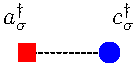
\includegraphics[width=2.5cm]{figures/c2_v1.pdf}
  \captionof{figure}[Minimal model]{Simple model and its corresponding normal order.}
  \label{amas_site_bain}
\end{minipage}
\begin{minipage}{0.7\textwidth}
  \centering
  \begin{align}
  \ket{i}
  \equiv
  \ket{
  n_{a\downarrow}
  n_{a\uparrow} 
  n_{\downarrow}
  n_{\uparrow}
  } 
  &= 
  (a_{\downarrow}^{\dag})^{n_{a\downarrow}}
  (a_{\uparrow}^{\dag})^{n_{a\uparrow}} 
  (c_{\downarrow}^{\dag})^{n_{\downarrow}}
  (c_{\uparrow}^{\dag})^{n_{\uparrow}} 
 \ket{0}
 \\
   &= 
  (a_{\downarrow}^{\dag})^{n_{a\downarrow}}
  (a_{\uparrow}^{\dag})^{n_{a\uparrow}}
  (c_{\downarrow}^{\dag})^{n_{\downarrow}}
  (c_{\uparrow}^{\dag})^{n_{\uparrow}} 
 \ket{0}_B \otimes 
 \ket{0}_c
 \\
   &= 
  (a_{\downarrow}^{\dag})^{n_{a\downarrow}}
  (a_{\uparrow}^{\dag})^{n_{a\uparrow}}
 \ket{0}_B \otimes 
  (c_{\downarrow}^{\dag})^{n_{\downarrow}}
  (c_{\uparrow}^{\dag})^{n_{\uparrow}} 
 \ket{0}_c
 \\
   &=  
  \ket{
  n_{a\downarrow}
  n_{a\uparrow} 
  }_B \otimes
  \ket{
  n_{\downarrow}
  n_{\uparrow}
  }_c
  \\
  &\equiv \ket{i_a} \otimes \ket{i_c}
  \label{ordrenormal0}
  \end{align}
  \vspace{-2em}
  %\captionof*{table}{Ordre des opérateurs de créations}
\end{minipage}
}

In its most simple form, a many body Hamiltonian can be expressed as:
\begin{align}
H &= \sum_{ij} \ket{i} \bra{j} H_{ij}
%H &= \sum_{ij} \ket{n_{a\downarrow}  n_{a\uparrow}  n_{\downarrow}  n_{\uparrow}} \bra{ n^{\prime}_{a\downarrow}  n^{\prime}_{a\uparrow}  n^{\prime}_{\downarrow}  n^{\prime}_{\uparrow}} H_{ij}
\label{eq::H_example}
\end{align}

For example, let's take a simple Anderson Impurity Model for this 2 sites model:
\begin{align}\label{AIM1}
H =&~U n_{\uparrow }n_{\downarrow}
- \theta \sum_{\sigma} (c_{\sigma }^{\dag}a_{\sigma} + a_{\sigma}^{\dag}c_{\sigma}
) 
+ \epsilon \sum_{\sigma} a_{\sigma }^{\dag}a_{\sigma}.
\end{align}

The matrix decomposion in Eq.~\eqref{eq::H_example} will give a big (16 by 16) matrix with a lot of zeros. If we permute rows and columns, we will obtain sectors (smaller matrices). The sectors found using this approach is:

\begin{align}
\begin{blockarray}{ccccc}
& \ket{0011} & \ket{0110} & \ket{1001} & \ket{1100} \\
\begin{block}{c(cccc)}
\bra{0011} & U & -\theta & \theta & 0\\
\bra{0110} & -\theta & \epsilon & 0 & -\theta\\
\bra{1001} & \theta & 0 & \epsilon & \theta\\
\bra{1100} & 0 & -\theta & \theta & 2\epsilon\\
\end{block}
\end{blockarray}
\end{align}

\begin{align}
\begin{blockarray}{cccc}
& & \ket{0001} & \ket{0100} \\ 
& & \ket{0010} & \ket{1000} \\
\begin{block}{cc(cc)}
\bra{0001}& \bra{0010} & 0 & \theta \\
\bra{0100}& \bra{1000} & \theta & \epsilon\\
\end{block}
\end{blockarray}
&&
\begin{blockarray}{cccc}
& & \ket{0111} & \ket{1101} \\ 
& & \ket{1011} & \ket{1110} \\
\begin{block}{cc(cc)}
\bra{0111}& \bra{1011} & U +\epsilon & -\theta \\
\bra{1101}& \bra{1110} & -\theta & 2\epsilon\\
\end{block}
\end{blockarray}
\end{align}

\begin{align}
\begin{blockarray}{cc}
& \ket{0000} \\
\begin{block}{c(c)}
\bra{0000} & 0\\
\end{block}
\end{blockarray}
&&
\begin{blockarray}{ccc}
& & \ket{1010} \\
& & \ket{0101} \\
\begin{block}{cc(c)}
\bra{1010} & \bra{0101} & 0\\
\end{block}
\end{blockarray}
&&
\begin{blockarray}{cc}
& \ket{1111} \\
\begin{block}{c(c)}
\bra{1111} & U + 2\epsilon \\
\end{block}
\end{blockarray}
\end{align}

This sector notation is similar to the information stored in TRIQS \Verb#atom_diag# function, except that in \Verb#atom_diag#, the matrices are not stored, but only their associated eigensystem.

Tracing over the bath of this Hamiltonian $H$ can be expressed as:
\begin{align}
\text Tr_B (H)
&= \sum_{k_a l_a} \sum_{ij} \braket{k_a}{i} \braket{j}{l_a} H_{ij}
%\\
%&= \sum_{k_a l_a} \sum_{ij} \braket{k_a}{i_a}\otimes\ket{i_c} \bra{j_c}\otimes \braket{j_a}{l_a}    H_{ij}
\\
&= \sum_{k_a l_a} \sum_{ij} \braket{k_a}{i_a}\braket{j_a}{l_a}    H_{ij} \ket{i_c} \bra{j_c}  
\end{align}

For the example here, this then give:
\begin{align}
\begin{blockarray}{ccccc}
& \ket{00}_c & \ket{01}_c & \ket{10}_c & \ket{10}_c \\
\begin{block}{c(cccc)}
\bra{00}_c & 4\epsilon &  &  & \\
\bra{01}_c &  & 4\epsilon &  & \\ 
\bra{10}_c &  &  & 4\epsilon & \\ 
\bra{11}_c &  &  &  & 4(U+\epsilon) \\ 
\end{block}
\end{blockarray}
\end{align}

({\color{red} Disclaimer: i am not sure about this factor 4, I think I miss a $\frac{1}{2^{N_{traced}} }$ somewhere.  My reasoning is that whatever the amount of baths that we consider here, the result should be similar.}) 

Now the extension for the propagator is straight forward. 

\begin{align}
U(\Delta\tau)
=
\text Tr_B (e^{-\Delta\tau H})
\end{align}

Of course, to take the exponential, we need first to diagonalize each block, take the exponential of the spectrum, reexpress the result in the original basis, then take the partial trace. 

This benchmark, although a little too simple, can be easily generalized to a bigger system. This is implemented in the new function $???$. The fundamental operator set should be defined such that the $N_?$ are not considere in the bath, and the parameter ??? will select up until with fundamental operator the system is not in the bath, the rest are, and will be traced out. 




%\bibliographystyle{apsrev4-1}
%\bibliography{inclus}



%merlin.mbs apsrev4-1.bst 2010-07-25 4.21a (PWD, AO, DPC) hacked
%Control: key (0)
%Control: author (72) initials jnrlst
%Control: editor formatted (1) identically to author
%Control: production of article title (-1) disabled
%Control: page (0) single
%Control: year (1) truncated
%Control: production of eprint (0) enabled
\begin{thebibliography}{1}%
\makeatletter
\providecommand \@ifxundefined [1]{%
 \@ifx{#1\undefined}
}%
\providecommand \@ifnum [1]{%
 \ifnum #1\expandafter \@firstoftwo
 \else \expandafter \@secondoftwo
 \fi
}%
\providecommand \@ifx [1]{%
 \ifx #1\expandafter \@firstoftwo
 \else \expandafter \@secondoftwo
 \fi
}%
\providecommand \natexlab [1]{#1}%
\providecommand \enquote  [1]{``#1''}%
\providecommand \bibnamefont  [1]{#1}%
\providecommand \bibfnamefont [1]{#1}%
\providecommand \citenamefont [1]{#1}%
\providecommand \href@noop [0]{\@secondoftwo}%
\providecommand \href [0]{\begingroup \@sanitize@url \@href}%
\providecommand \@href[1]{\@@startlink{#1}\@@href}%
\providecommand \@@href[1]{\endgroup#1\@@endlink}%
\providecommand \@sanitize@url [0]{\catcode `\\12\catcode `\$12\catcode
  `\&12\catcode `\#12\catcode `\^12\catcode `\_12\catcode `\%12\relax}%
\providecommand \@@startlink[1]{}%
\providecommand \@@endlink[0]{}%
\providecommand \url  [0]{\begingroup\@sanitize@url \@url }%
\providecommand \@url [1]{\endgroup\@href {#1}{\urlprefix }}%
\providecommand \urlprefix  [0]{URL }%
\providecommand \Eprint [0]{\href }%
\providecommand \doibase [0]{http://dx.doi.org/}%
\providecommand \selectlanguage [0]{\@gobble}%
\providecommand \bibinfo  [0]{\@secondoftwo}%
\providecommand \bibfield  [0]{\@secondoftwo}%
\providecommand \translation [1]{[#1]}%
\providecommand \BibitemOpen [0]{}%
\providecommand \bibitemStop [0]{}%
\providecommand \bibitemNoStop [0]{.\EOS\space}%
\providecommand \EOS [0]{\spacefactor3000\relax}%
\providecommand \BibitemShut  [1]{\csname bibitem#1\endcsname}%
\let\auto@bib@innerbib\@empty
%</preamble>
\bibitem [{\citenamefont {Boag}\ \emph {et~al.}()\citenamefont {Boag},
  \citenamefont {Gull},\ and\ \citenamefont
  {Cohen}}]{boag_inclusion-exclusion_2018}%
  \BibitemOpen
  \bibfield  {author} {\bibinfo {author} {\bibfnamefont {A.}~\bibnamefont
  {Boag}}, \bibinfo {author} {\bibfnamefont {E.}~\bibnamefont {Gull}}, \ and\
  \bibinfo {author} {\bibfnamefont {G.}~\bibnamefont {Cohen}},\ }\href
  {\doibase 10.1103/PhysRevB.98.115152} {\ \textbf {\bibinfo {volume} {98}},\
  \bibinfo {pages} {115152}}\BibitemShut {NoStop}%
\end{thebibliography}%



\end{document}












































From Michel's notes:

\begin{align}
Z &=Z_{\text {bath }} \int D d_{a \alpha} D d_{a \alpha}^{\dagger} T_{\tau} \exp \left(-S_{\text {tot }}\right) \\
&=Z_{\text {bath }} \int D d_{a \alpha} D d_{a \alpha}^{\dagger} T_{\tau} \exp \left(-S_{\text {loc }}\right) \prod_{a} T_{\tau} \exp \left(-S_{a}\right)
\end{align}


\begin{align}
S_{a}=\sum_{\alpha, \beta} \int d \tau d \tau^{\prime} d_{a \alpha}^{\dagger}(\tau) \Delta_{\alpha \beta}^{a}\left(\tau-\tau^{\prime}\right) d_{a \beta}\left(\tau^{\prime}\right)
\end{align}

\begin{align}
Z=& Z_{\text {bath }} \int D d_{a \alpha} D d_{a \alpha}^{\dagger} T_{\tau} \exp \left(-S_{\text {loc }}\right) \prod_{a} T_{\tau} \sum_{n_{a}} \frac{(-1)^{n_{a}}}{n_{a} !} \int_{0}^{\beta} d \tau_{a 1} d \tau_{a 1}^{\prime} \cdots d \tau_{a n} d \tau_{a n}^{\prime} \\
& \sum_{\alpha_{1}^{a} \ldots \beta_{n_{a}}^{a}} d_{a \alpha_{1}^{a}}^{\dagger}\left(\tau_{a 1}\right) \Delta_{\alpha_{1}^{2} \beta_{1}^{a}}^{a}\left(\tau_{a 1}-\tau_{a 1}^{\prime}\right) d_{a \beta_{1}^{a}}\left(\tau_{a 1}^{\prime}\right) \cdots \\
& d_{a \alpha_{n_{a}}^{\dagger}}^{\dagger}\left(\tau_{a n_{a}}\right) \Delta_{\alpha_{n_{a}}^{a} \beta_{n_{a}}^{a}}\left(\tau_{a n_{a}}-\tau_{a n_{a}}^{\prime}\right) d_{a \beta_{n_{a}}^{a}}\left(\tau_{a n_{a}}^{\prime}\right)
\end{align}

\begin{align}
Z=& Z_{\text {bath }} \int D d_{a \alpha} D d_{a \alpha}^{\dagger} T_{\tau} \exp \left(-S_{\text {loc }}\right) \prod_{a} T_{\tau} \sum_{n_{a}} \frac{(-1)^{n_{a}}}{n_{a} !} \int_{0}^{\beta} d \tau_{a 1}^{\prime} \cdots d \tau_{a n}^{\prime} \\
& \int_{0}^{\beta} d \tau_{a 1} \int_{0}^{\tau_{a 1}} d \tau_{a 2} \cdots \sum_{\alpha_{1}^{a} \ldots \beta_{n_{a}}^{a}} d_{a \alpha_{1}^{a}}^{\dagger}\left(\tau_{a 1}\right) d_{a \beta_{1}^{a}}\left(\tau_{a 1}^{\prime}\right) \cdots \\
& d_{a \alpha_{n a}^{a}}^{\dagger}\left(\tau_{a n_{a}}\right) d_{a \beta_{n_{a}}^{a}}\left(\tau_{a n_{a}}^{\prime}\right) \operatorname{Det} M_{a}^{-1}
\end{align}

\begin{align}
Z=& Z_{\text {bath }} \int D d_{a \alpha} D d_{a \alpha}^{\dagger} T_{\tau} \exp \left(-S_{\text {loc }}\right) \prod_{a} T_{\tau} \sum_{n_{a}}(-1)^{n_{a}} \int_{0}^{\beta} d \tau_{a 1}^{\prime} \int_{0}^{\tau_{a 1}^{\prime}} d \tau_{a 2}^{\prime} \cdots \\
& \int_{0}^{\beta} d \tau_{a 1} \int_{0}^{\tau_{a 1}} d \tau_{a 2} \cdots \sum_{\alpha_{1}^{a} \ldots \beta_{n_{a}}^{a}} d_{a \alpha_{1}^{a}}^{\dagger}\left(\tau_{a 1}\right) d_{a \beta_{1}^{a}}\left(\tau_{a 1}^{\prime}\right) \cdots \\
& d_{a \alpha_{n_{a}}^{a}}^{\dagger}\left(\tau_{a n_{a}}\right) d_{a \beta_{n_{a}}^{a}}\left(\tau_{a n_{a}}^{\prime}\right) \operatorname{Det} M_{a}^{-1}
\end{align}

